\documentclass[12pt]{article}

\usepackage[a4paper,margin=2cm,footskip=.5cm]{geometry}
\usepackage{amsmath}
\usepackage{commath}

\usepackage{indentfirst}
\usepackage{subscript}

\usepackage{fontspec}	
\usepackage{unicode-math}

\setmainfont[Ligatures=TeX]{Palatino} % Georgia
\setmathfont{xits-math.otf} % Cambria Math

\usepackage{algorithm, algpseudocode}
\newfontfamily\codefont{Consolas} % Inconsolata
\newfontfamily\commentfont[Color={888888}]{Consolas}
\makeatletter
\renewcommand{\ALG@beginalgorithmic}{\codefont}
\makeatother
\algrenewcommand{\algorithmiccomment}[1]{\hfill \commentfont \# #1 \codefont}

\usepackage{graphicx}

%----------------------------------------------------

\begin{document}

\section{Lecture 2: Pattern Discovery Basic Concepts}
\subsection{Frequent Itemsets (Patterns)}

X = itemset

\begin{itemize}
\item \textbf{(absolute) support (count) of X:} Frequency or the number of occurrences of an itemset X
\item \textbf{(relative) support, s:} The fraction of transactions that contains X (i.e., the probability that a transaction contains X)
\item An itemset X is \textbf{frequent} if the support of X is no less than a $minsup$ threshold (denoted as $\sigma$)
\end{itemize}

%--
\subsection{Association Rules}
Association rules: $X \to Y (s, c)$:
\begin{itemize}
\item \textbf{Support}, s: The probability that a transaction contains $X \cup Y$
\item \textbf{Confidence}, c: The conditional probability that a transaction containing X also contains Y: 
\begin{equation*}
c = \frac{sup(X \cup Y)}{sup(X)}
\end{equation*}
\end{itemize}

%--
\subsection{Expressing Patterns in Compressed Form}
Solution 1: \textbf{Closed patterns:} \textit{A pattern (itemset) X is closed if X is frequent, and there exists no super-pattern $Y \supset X$, with the same support as X}.\\
    
Closed pattern is a lossless compression of frequent patterns.\\

Solution 2: \textbf{Max-patterns:} \textit{A pattern X is a max-pattern if X is frequent and there exists no frequent super-pattern $Y \supset X$}.\\

Max-pattern is a lossy compression!

%--
\subsection{Recommended readings}
\begin{itemize}
\item R. Agrawal, T. Imielinski, and A. Swami, <<Mining association rules between sets of items in large databases>>, in Proc. of SIGMOD'93
\item R. J. Bayardo, <<Efficiently mining long patterns from databases>>, in Proc. of SIGMOD'98
\item N. Pasquier, Y. Bastide, R. Taouil, and L. Lakhal, <<Discovering frequent closed itemsets
for association rules>>, in Proc. of ICDT'99
\item J. Han, H. Cheng, D. Xin, and X. Yan, <<Frequent Pattern Mining: Current Status and Future Directions>>, Data Mining and Knowledge Discovery, 15(1): 55-86, 2007
\end{itemize}

\section{Lecture 3. Efficient Pattern Mining Methods}
\subsection{The Downward Closure Property of Frequent Patterns}
The downward closure (also called <<Apriori>>) property of frequent patterns: \textbf{Any subset of a frequent itemset must be frequent}. Apriori pruning principle: \textbf{If there is any itemset which is infrequent, its superset should not even be generated!}\\

Scalable mining Methods: Three major approaches
\begin{itemize}
\item Level-wise, join-based approach: Apriori (\ref{apriori})
\item Vertical data format approach: Eclat (\ref{eclat})
\item Frequent pattern projection and growth: FPgrowth (\ref{fpgrowth})
\end{itemize}

%--
\subsection{The Apriori Algorithm}\label{apriori}
\subsubsection{Algorithm pseudocode}
$C_k$: Candidate itemset of size k

$F_k$ : Frequent itemset of size k

TDB = transactional database\\

\begin{algorithm}
\caption{The Apriori Algorithm}
\begin{algorithmic}
\State $k := 1$
\State $F_k :=$ frequent items \Comment{frequent 1-itemset}
\While{$F_k \neq \varnothing$}
    \State $C_{k+1} :=$ candidates generated from $F_k$ \Comment{candidate generation}
    \State Derives $F_{k+1}$ by counting candidates in $C_{k+1}$ with respect to TDB at minsup
    \State $k := k + 1$
\EndWhile
\State \Return $\cup_k F_k$  \Comment{return F\textsubscript{k} generated at each level}
\end{algorithmic}
\end{algorithm}

%--
\subsubsection{How to generate candidates?}

\begin{itemize}
\item Step1: self-joining F\textsubscript{k}
\item Step2: pruning
\end{itemize}


\begin{algorithm}
\caption{Step1: self-joining F\textsubscript{k}}
\begin{algorithmic}
\State insert into C\textsubscript{k}
\State select p.item\textsubscript{1}, p.item\textsubscript{2}, ..., p.item\textsubscript{k-1}, q.item\textsubscript{k-1}
\State from F\textsubscript{k-1} as p, F\textsubscript{k-1} as q
\State where p.item\textsubscript{1}= q.item\textsubscript{1}, ..., p.item\textsubscript{k-2} = q.item\textsubscript{k-2}, p.item\textsubscript{k-1} < q.item\textsubscript{k-1}
\end{algorithmic}
\end{algorithm}

\begin{algorithm}
\caption{Step2: pruning}
\begin{algorithmic}
\ForAll{itemsets c in C\textsubscript{k}}
    \ForAll{(k-1) subsets s of c}
        \If{s is not in F\textsubscript{k-1}}
            \State delete c from C\textsubscript{k}
        \EndIf
    \EndFor
\EndFor
\end{algorithmic}
\end{algorithm}    

%--    
\subsection{Extensions or Improvements of Apriori}
\begin{itemize}
\item Reduce passes of transaction database scans 
    \begin{itemize}
    \item Partitioning
    \item Dynamic itemset counting
    \end{itemize}
\item Shrink the number of candidates
    \begin{itemize}
    \item Hashing
    \item Pruning by support lower bounding
    \item Sampling
    \end{itemize}
\item Exploring special data structures
    \begin{itemize}
    \item Tree projection
    \item H-miner
    \item Hypecube decomposition
    \end{itemize}
\end{itemize}  

%--
\subsubsection{Partitioning}
Theorem: \textit{Any itemset that is potentially frequent in TDB must be frequent in at least one of the partitions of TDB}\\

Method: Scan Database Only Twice:
\begin{itemize}
\item Scan 1: Partition database (how?) and find local frequent patterns
\item Scan 2: Consolidate global frequent patterns (how to?)
\end{itemize}

%--
\subsubsection{Direct Hashing and Pruning (DHP)}
Observation: \textit{A k-itemset whose corresponding hashing bucket count is below the threshold cannot be frequent}

%-- 
\subsection{Vertical Data Format}\label{eclat}
\textbf{ECLAT} - Equivalence Class Transformation

Frequent patterns are derived based on vertical intersections. To accelerate data mining you can use \textbf{diffset}: only keep track of differences of tids.

%--
\subsection{A Pattern Growth Approach}\label{fpgrowth}
\textbf{FP-tree} - frequent pattern tree

\begin{figure}[h!]
    \centering
    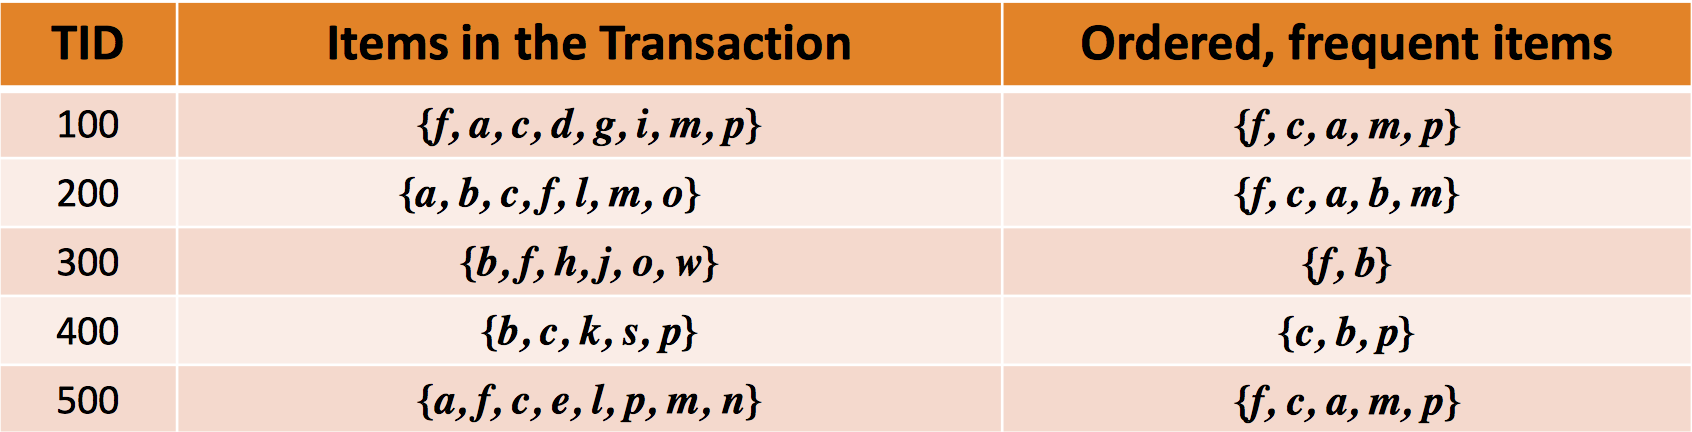
\includegraphics[width=\linewidth]{transactional_db.png}
    \caption{Transational DB}
\end{figure}

\begin{figure}[h!]
    \centering
    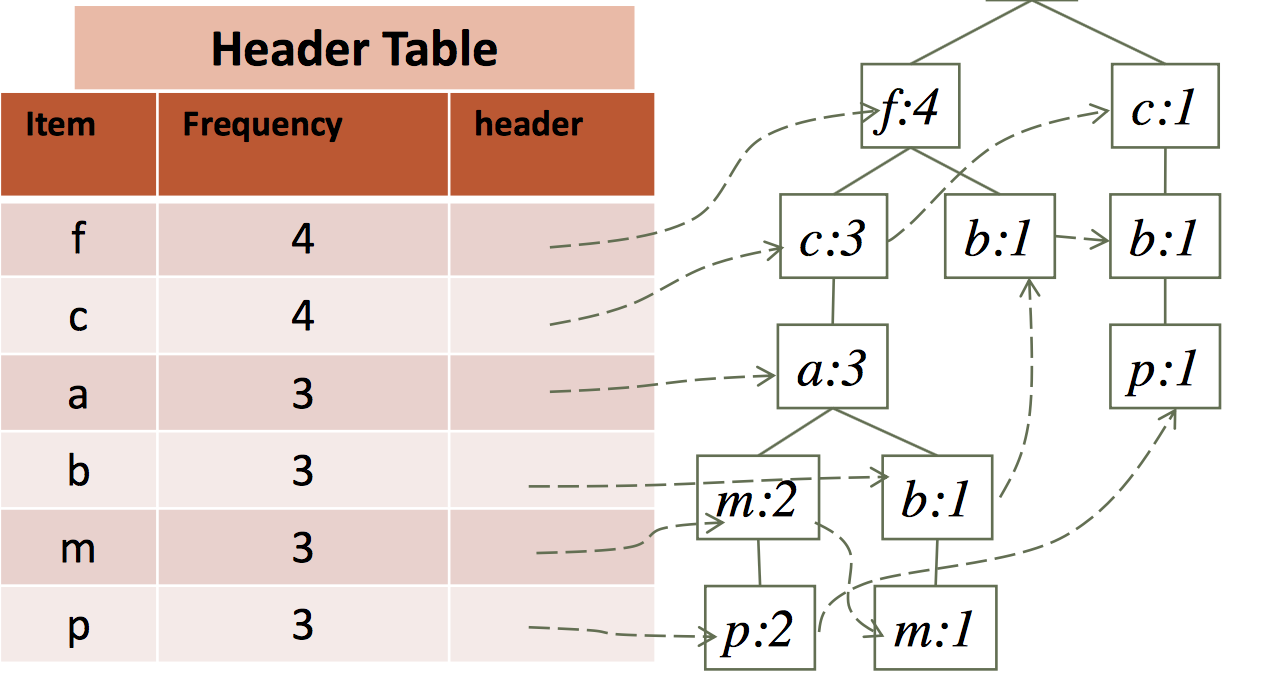
\includegraphics[width=\linewidth]{fptree.png}
    \caption{FP-tree}
\end{figure}

%--
\subsection{CLOSET+: Mining Closed Itemsets by Pattern-Growth}
Itemset merging: \textit{If Y appears in every occurrence of X, then Y
is merged with X}

%--
\subsection{Recommended readings}
\begin{itemize}
\item R. Agrawal and R. Srikant, <<Fast algorithms for mining association rules>>, VLDB'94
\item A. Savasere, E. Omiecinski, and S. Navathe, <<An efficient algorithm for mining association rules in large
databases>>, VLDB'95
\item J. S. Park, M. S. Chen, and P. S. Yu, <<An effective hash-based algorithm for mining association rules>>, SIGMOD'95
\item S. Sarawagi, S. Thomas, and R. Agrawal, <<Integrating association rule mining with relational database systems: Alternatives and implications>>, SIGMOD'98
\item M. J. Zaki, S. Parthasarathy, M. Ogihara, and W. Li, <<Parallel algorithm for discovery of association rules>>, Data Mining and Knowledge Discovery, 1997
\item J. Han, J. Pei, and Y. Yin, <<Mining frequent patterns without candidate generation>>, SIGMOD’00
\item M. J. ZakiandHsiao, <<CHARM: An Efficient Algorithm for Closed Itemset Mining>>, SDM'02
\item J. Wang, J. Han, and J. Pei, <<CLOSET+: Searching for the Best Strategies for Mining Frequent Closed Itemsets>>, KDD'03
\item C. C. Aggarwal, M.A., Bhuiyan, M. A. Hasan, <<Frequent Pattern Mining Algorithms: A Survey>>, in Aggarwal and Han (eds.): Frequent Pattern Mining, Springer, 2014
\end{itemize}
\section{Lecture 4: Pattern Evaluation}

\subsection{Interestingness Measures: Lift and $\mathbf{\chi ^2}$}

\subsubsection{Interestingness Measure: Lift}

\textbf{Lift} - measure of dependent/correlated events:
\begin{equation*}
\mathrm{lift}(B,C) = \frac{c(B \to C)}{s(C)} = \frac{s(B \cup C)}{s(B) \times s(C)}
\end{equation*}

Lift(B, C) may tell how B and C are correlated:
\begin{itemize}
\item $\mathrm{Lift}(B, C) = 1$: B and C are independent
\item $\mathrm{Lift}(B, C) > 1$: positively correlated
\item $\mathrm{Lift}(B, C) < 1$: negatively correlated
\end{itemize}

%--
\subsubsection{Interestingness Measure: $\mathbf{\chi ^2}$}
\begin{equation*}
\chi^2=\sum\frac{(Observed-Expected)^2}{Expected}
\end{equation*}

General rules:
\begin{itemize}
\item $\chi^2 = 0$: independent
\item $\chi^2 > 0$: correlated, either positive or negative, so it needs additional test
\end{itemize}

Too many null transactions may lead to invalid correlation result!

\subsection{Null Invariance Measures}

\begin{gather*}
\mathrm{AllConf}(A, B) = \frac{s(A \cup B)}{\max\{s(A), s(B)\}} \\
\mathrm{Jaccard}(A, B) = \frac{s(A \cup B)}{s(A) + s(B) - s(A \cup B)} \\
\mathrm{Cosine}(A, B) = \frac{s(A \cup B)}{\sqrt{s(A) \times s(B)}} \\
\mathrm{Kulczynsky}(A, B) = \frac{1}{2}\left(\frac{s(A \cup B)}{s(A)} + \frac{s(A \cup B)}{s(B)}\right)\\
\mathrm{MacConf}(A, B)=\max\left\{\frac{s(A)}{s(A \cup B)}, \frac{s(B)}{s(A \cup B)}\right\}
\end{gather*}

\subsection{Imbalance Ratio}
IR (Imbalance Ratio): measure the imbalance of two itemsets A and B in rule implications:
\begin{equation*}
\mathrm{IR}(A, B)=\frac{\abs{s(A)-s(B)}}{s(A) + s(B) - s(A \cup B)}
\end{equation*}

Kulczynski and Imbalance Ratio (IR) together present a clear picture

\subsection{Recommended Readings}
\begin{itemize}
\item C. C. Aggarwal and P. S. Yu. A New Framework for Itemset Generation. PODS’98
\item S. Brin, R. Motwani, and C. Silverstein. Beyond market basket: Generalizing
association rules to correlations. SIGMOD'97
\item M. Klemettinen, H. Mannila, P. Ronkainen, H. Toivonen, and A. I. Verkamo. Finding interesting rules from large sets of discovered association rules. CIKM'94
\item E. Omiecinski. Alternative Interest Measures for Mining Associations. TKDE’03
\item P.-N. Tan, V. Kumar, and J. Srivastava. Selecting the Right Interestingness Measure for
Association Patterns. KDD'02
\item T. Wu, Y. Chen and J. Han, Re-Examination of Interestingness Measures in Pattern Mining: A Unified Framework, Data Mining and Knowledge Discovery, 21(3):371-397, 2010
\end{itemize}
\section{Lecture 4: Mining Diverse Patterns}

\subsection{Mining Multi-Level Associations}

Items often form hierarchies. How to set min-support thresholds? \textbf{Level-reduced min-support}: items at the lower level are expected to have lower support.\\

Efficient mining: \textbf{shared} multi-level mining. Use the lowest min-support to pass down the set of candidates.\\

Redundancy\footnote{Redundancy - избыточность} filtering: some rules may be redundant due to <<ancestor>>\footnote{Ancestor -- предок} relationships between items. A rule is \textbf{redundant} if:
\begin{itemize}
\item its support is close to the <<expected>> value, according to its <<ancestor>> rule
\item it has a similar confidence as its <<ancestor>>.
\end{itemize}\\

It is necessary to have customized min-support settings for different kinds of items: group-based <<individualized>> min-support.

%--
\subsection{Mining Multi-Dimensional Associations}
Rules can be single-dimensional or multi-dimensional:
\begin{itemize}
\item Single-dimentional: 
\begin{equation*}
\mathrm{buys}(X, \text{<<milk>>}) \Rightarrow \mathrm{buys}(X, \text{<<bread>>})
\end{equation*}
\item Inter-dimension association rule: 
\begin{equation*}
\mathrm{age}(X, \text{<<18-25>>}) \wedge \mathrm{occupation}(X, \text{<<student>>}) \Rightarrow \mathrm{buys}(X, \text{<<coke>>})
\end{equation*}
\item Hybrid-dimension association rules: 
\begin{equation*}
\mathrm{age}(X, \text{<<18-25>>}) \wedge \mathrm{buys}(X, \text{<<popcorn>>}) \Rightarrow \mathrm{buys}(X, \text{<<coke>>})
\end{equation*}
\end{itemize}


Attributes can be categorical or numerical

%--    
\subsection{Mining Quantitative Associations}

Methods:
\begin{itemize}
\item Static discretization based on predefined concept hierarchies
\item Dynamic discretization based on data distribution
\item Clustering: distance-based association
\item Deviation analysis
\end{itemize}

%--
\subsection{Mining Negative Correlations}
\begin{itemize}
\item Rare patterns = very low support but interesting
\item Negative patterns = negatively correlated, unlikely to happen together
\end{itemize}

A support-based definition: if itemsets A and B are both frequent but rarely occur together, i.e., $\sup(A \cup B) << \sup (A) \times \sup(B)$ then A and B are negatively correlated.\\

The support-based definition is not null-invariant!\\

A Kulczynski measure-based definition: if itemsets A and B are frequent but $\frac{P(A \mid B) + P(B \mid A)}{2} < \varepsilon$, where $\varepsilon$ is a negative pattern threshold, then A and B are negatively correlated.

%--
\subsection{Mining Compressed Patterns}
\subsubsection{Mining Compressed Patterns}
Pattern distance measure:
\begin{equation*}
Dist(P_1, P_2)=1-\frac{\abs{T(P_1) \cap T(P_2)}}{\abs{T(P_1) \cup T(P_2)}}
\end{equation*}

\textbf{$\mathbf{\delta}$-clustering}. For each pattern P, find all patterns which can be expressed by P and whose distance to P is within $\delta$ ($\delta$-cover). All patterns in the cluster can be represented by P = compressed patterns.\footnote{Method for efficient, direct mining of compressed frequent patterns: Xin et al., VLDB’05.}

\subsubsection{Redundancy-Aware Top-k Patterns}

\begin{figure}[h]
\centering
\subfigure[a set of patterns]{%
  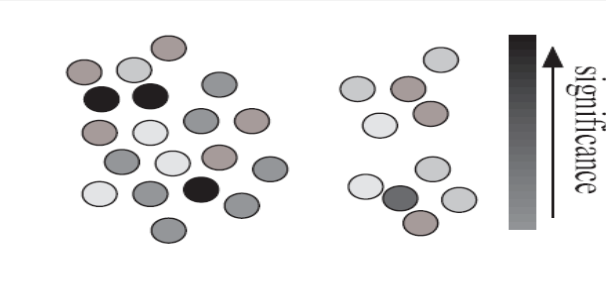
\includegraphics[width=0.32\linewidth, height=0.2\linewidth]{desired_patterns_1.png}
  \label{fig:desired1}}
\quad
\subfigure[redundancy-aware top-k]{%
  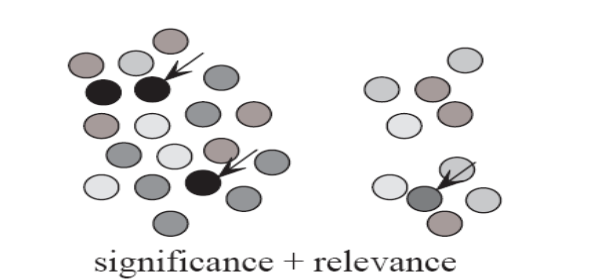
\includegraphics[width=0.32\linewidth, height=0.2\linewidth]{desired_patterns_2.png}
  \label{fig:desired2}}
\subfigure[traditional top-k]{%
  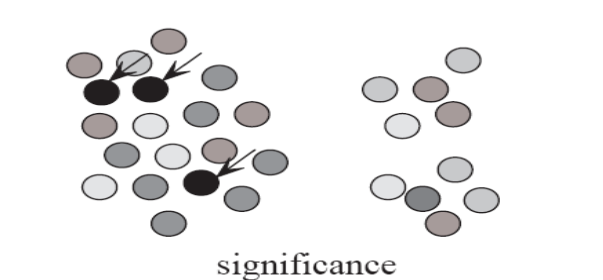
\includegraphics[width=0.32\linewidth, height=0.2\linewidth]{desired_patterns_3.png}
  \label{fig:desired3}}
\quad
\subfigure[summarization]{%
  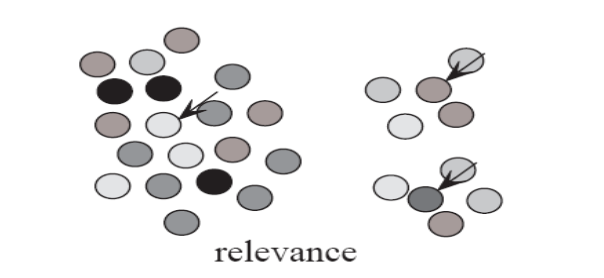
\includegraphics[width=0.32\linewidth, height=0.2\linewidth]{desired_patterns_4.png}
  \label{fig:desired4}}
%
\caption{Desired patterns: high significance \& low redundancy}
\label{fig:desired}
\end{figure}

Use \textbf{MMS (Maximal Marginal Significance)} for measuring the combined significance of a pattern set.\footnote{Xin et al., Extracting Redundancy-Aware Top-K Patterns, KDD’06.}

%--
\subsection{Mining Colossal Patterns}
\subsubsection{Pattern-Fusion}
\textbf{Pattern fusion strategy:} fuse small patterns together in one step to generate new pattern candidates of significant sizes.\\

Subpatterns $\alpha_1$ to $\alpha_k$ cluster tightly around the colossal pattern $\alpha$ by sharing a similar support. Such subpatterns are \textbf{core patterns} of $\alpha$. A colossal pattern can be generated by merging a set of core patterns.

\subsubsection{Robustness of Colossal Patterns}
\begin{definition}
For a frequent pattern $\alpha$, a subpattern $\beta$ is a $\mathbf{\tau}$\textbf{-core pattern} of $\alpha$ if $\beta$ shares a similar support set with $\alpha$, i.e., 
\begin{equation*}
\frac{\abs{D_\alpha}}{\abs{D_\beta}} \geqslant \tau, 0 < \tau \leqslant 1, 
\end{equation*}
where $\tau$ is called the \textbf{core ratio}.
\end{definition}

\begin{definition}
\textbf{$\mathbf{(d, \tau)}$-robustness}\footnote{Robustness - прочность}: a pattern $\alpha$ is $(d, \tau)$-robust if d is the maximum number of items that can be removed from $\alpha$ for the resulting pattern to remain a $\tau$-core pattern of $\alpha$:
\begin{equation*}
d = \max_{\beta}\{\abs{\alpha} - \abs{\beta} \mid \beta \subseteq \alpha\text{, and }\beta\text{ is a }\tau\text{-core pattern of }\alpha\}
\end{equation*}
\end{definition}

For a pattern $\alpha$ let $C_\alpha$ be the set of all its core patterns for a specified $\tau$:
\begin{equation*}
C_\alpha = \{\beta \mid \beta \subseteq \alpha, \frac{\abs{D_\alpha}}{\abs{D_\beta}} \geqslant \tau\}
\end{equation*}

\begin{theorem}
For a $(d, \tau)$-robust pattern $\alpha$:
\begin{equation*}
\abs{C_\alpha} \geqslant 2^d
\end{equation*}
\end{theorem}

\textbf{Robustness of Colossal Patterns}: a colossal pattern tends to have
much more core patterns than small patterns. Such core patterns can be clustered together to form <<dense balls>> based on pattern distance defined by 
\begin{equation*}
Dist(\alpha, \beta)=1-\frac{\abs{D_\alpha \cap D_\beta}}{\abs{D_\alpha \cup D_\beta}}
\end{equation*}

\begin{theorem}
For two patterns $\beta_1, \beta_2 \in C_\alpha$ 
\begin{equation*}
Dist(\beta_1, \beta_2) \leqslant r(\tau)\text{, where }r(\tau)=1-\frac{1}{2/\tau-1}
\end{equation*}
\end{theorem}

\subsubsection{The Pattern-Fusion Algorithm}
\begin{itemize}
\item Initialization (Creating initial pool): Use an existing algorithm to mine all frequent patterns up to a small size, e.g., 3
\item Iteration (Iterative Pattern Fusion):
\begin{itemize}
\item At each iteration, K seed patterns are randomly picked from the current pattern
pool
\item For each seed pattern thus picked, we find all the patterns within a bounding ball centered at the seed pattern
\item All these patterns found are fused together to generate a set of super-patterns
\item All the super-patterns thus generated form a new pool for the next iteration
\end{itemize}
\item Termination: when the current pool contains no more than K patterns at the beginning of an iteration
\end{itemize}

%--
\subsection{Recommended Readings}
\begin{itemize}
\item R. Srikant and R. Agrawal, <<Mining generalized association rules>>, VLDB'95
\item Y. Aumann and Y. Lindell, <<A Statistical Theory for Quantitative Association Rules>>, KDD'99
\item D. Xin, J. Han, X. Yan and H. Cheng, <<On Compressing Frequent Patterns>>, Knowledge and Data Engineering, 60(1): 5-29, 2007
\item D. Xin, H. Cheng, X. Yan, and J. Han, <<Extracting Redundancy-Aware Top-K Patterns>>, KDD'06
\item F. Zhu, X. Yan, J. Han, P. S. Yu, and H. Cheng, <<Mining Colossal Frequent Patterns by Core Pattern Fusion>>, ICDE'07
\item J. Han, H. Cheng, D. Xin, and X. Yan, <<Frequent Pattern Mining: Current Status and Future Directions>>, Data Mining and Knowledge Discovery, 15(1): 55-86, 2007
\end{itemize}
\section{Constraint-Based Pattern Mining}
\subsection{Meta-Rule Guided Mining}
In general, (meta) rules can be in the form of
\begin{equation*}
P_1 \wedge P_2 \wedge ... \wedge P_l \Rightarrow Q_1 \wedge Q_2 \wedge ... \wedge Q_r
\end{equation*}

Method to find meta-rules:
\begin{itemize}
\item Find frequent (l + r) predicates (based on min-support)
\item Push constants deeply when possible into the mining process
\item Also, push min\_conf, min\_correlation, and other measures as early as possible (measures acting as constraints)
\end{itemize}

%--
\subsection{Kinds of Constraints}
\begin{itemize}
\item Pattern space pruning constraints
\begin{itemize}
\item Anti-monotonic: If constraint c is violated, its further mining can be terminated
\item Monotonic: If c is satisfied, no need to check c again
\item Succinct\footnote{Succinct - краткий}: if the constraint c can be enforced by directly manipulating the data
\item Convertible: c can be converted to monotonic or anti-monotonic if items can be properly ordered in processing
\end{itemize}
\item Data space pruning constraints
\begin{itemize}
\item Data succinct: Data space can be pruned at the initial pattern mining process
\item Data anti-monotonic: If a transaction t does not satisfy c, then t can be pruned to reduce data processing effort
\end{itemize}
\end{itemize}

Anti-monotonic constraints have more pruning power than monotonic constraints.

\subsubsection{Pattern space pruning constraints}
Constraint c is \textbf{anti-monotone}: if an itemset S violates constraint \textbf{c}, so does any of its superset. That is, mining on itemset S can be terminated. For example, constraint $\sup(S) \geqslant \sigma$ is anti-monotone.\\

A constraint c is \textbf{monotone}: if an itemset S satisfies the constraint \textbf{c}, so does any of its superset. That is, we do not need to check \textbf{c} in subsequent mining. For example, constraints $\sum(S.price) \geqslant v$ or $\min(S.price) \leqslant v$ are monotone.

\subsubsection{Data space pruning constraints}
A constraint \textbf{c} is \textbf{data anti-monotone}: if a data entry \textbf{t} cannot satisfy a pattern \textbf{p} under constraint \textbf{c}, \textbf{t} cannot satisfy \textbf{p}’s superset either. That's why, data entry \textbf{t} can be pruned.\\

\textbf{Succinctness}: if the constraint \textbf{c} can be enforced by directly manipulating the data.\\

\textbf{Convertible constraints}: convert tough\footnote{Tough - жесткий} constraints into (anti-)monotone by proper ordering of items in transactions. For example, ordering items in value-descending order makes the constraint $avg(S.profit) > 20$ anti-monotone \textit{if the patterns grow in the right order}.

%--
\subsection{Recommended Readings}
\begin{itemize}
\item R. Srikant, Q. Vu, and R. Agrawal, <<Mining association rules with item constraints>>, KDD'97
\item R. Ng, L.V.S. Lakshmanan, J. Han \& A. Pang, Exploratory mining and pruning optimizations of constrained association rules>>, SIGMOD’98
\item G. Grahne, L. Lakshmanan, and X. Wang, <<Efficient mining of constrained correlated sets>>, ICDE'00
\item J. Pei, J. Han, and L. V. S. Lakshmanan, <<Mining Frequent Itemsets with Convertible Constraints>>, ICDE'01
\item J. Pei, J. Han, and W. Wang, <<Mining Sequential Patterns with Constraints in Large Databases>>, CIKM'02
\item F. Bonchi, F. Giannotti, A. Mazzanti, and D. Pedreschi, <<ExAnte: Anticipated Data Reduction in Constrained Pattern Mining>>, PKDD'03
\item F. Zhu, X. Yan, J. Han, and P. S. Yu, <<gPrune: A Constraint Pushing Framework for Graph Pattern Mining>>, PAKDD'07
\end{itemize}


\end{document}
